\section{Markov decision process}

Markov decision processes adhere to Markov property: 
\begin{property}
    The future state ($s^\prime$) and reward ($r$) only depend on current state ($s$) and action ($a$)
\end{property}
It is not a limiting assumption, it can be seen as a
property of state 

\paragraph*{One-step dynamic}
In a Markov Decision Process (MDP), the one-step dynamic can be described as:
\[p(s^\prime,r|s,a)\]
That is defined on: $p:\mathcal{S}\times\mathcal{R}\times\mathcal{S}\times\mathcal{A}\rightarrow\left[0,1\right]$. 
The main property is that: 
\[\sum_{s^\prime\in\mathcal{S}}\sum_{r\in\mathcal{R}}p(s^\prime,r|s,a)=1\qquad \forall s \in \mathcal{S},\forall a\in\mathcal{A}(s)\]

\subsection{Finite Markov decision processes}
When the Markov Property holds and both the state and action sets are finite, the problem is termed as a finite Markov Decision Process. 
To formally define a finite MDP, it's necessary to specify the following: sets for states and actions, and one-step dynamics:
\[p(s^\prime, r | s, a) = \Pr\{S_{t+1}=s^\prime, R_{t+1}=r | S_t=s, A_t=a\}\]
We can further deduce the distribution of the next state and the expected reward: 
The overarching formulation is as follows:
\begin{align*}
    &p(s^\prime | s, a) \doteq \Pr\{S_{t+1} = s^\prime | S_t = s, A_t = a\} = \sum_{r \in \mathcal{R}} p(s^\prime, r | s, a) \\
    &r(s, a) \doteq \mathbb{E}\left[R_{t+1} | S_t = s, A_t = a\right] = \sum_{r \in \mathcal{R}} r \sum_{s^\prime \in \mathcal{S}} p(s^\prime, r | s, a) 
\end{align*}

\paragraph*{Return}
The agent should refrain from selecting actions solely based on immediate rewards. 
Instead, prioritizing long-term consequences over short-term gains is crucial. 
Hence, it's imperative to consider the sequence of future rewards. 
To this end, we define the return, $G_t$, as a function of the sequence of future rewards.
\[G_t \doteq f\left(R_{t+1}+R_{t+2}+R_{t+3}+\cdots\right)\]
To achieve success, the agent must aim to maximize the expected return, denoted as $\mathbb{E}\left[G_t\right]$. 
Various definitions of return are conceivable, including: total reward, discounted reward, or average reward. 

\paragraph*{Episodic task}
In episodic task the agent-environment interaction naturally breaks into chunks called episodes.
\begin{figure}[H]
    \centering
    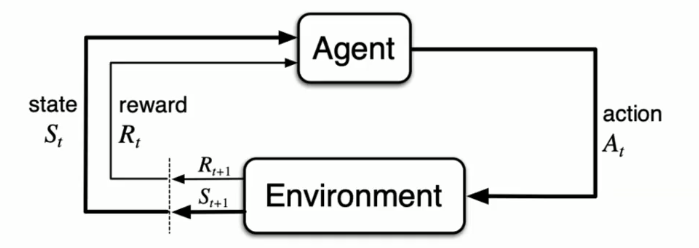
\includegraphics[width=0.75\linewidth]{images/rl.png}
    \caption{Markov decision processes episodic tasks}
\end{figure}
It is possible to maximize the expected total reward:
\[\mathbb{E}\left[G_t\right]=\mathbb{E}\left[R_{t+1}+R_{t+2}+R_{t+3}+\cdots+R_T\right]\]

\paragraph*{Continuing tasks}
In continuing task the agent-environment interaction goes on continually and
there are no terminal state
The total reward is a sum over an infinite sequence and might not be finite:
\[G_t\doteq R_{t+1}+R_{t+2}+R_{t+3}+\cdots+R_{t+k}+\cdots\overset{?}{=}\infty\]
To solve this issue we can discount the future rewards by a factor $\gamma$ ($0 < \gamma < 1$):
\[G_t\doteq R_{t+1}+\gamma R_{t+2}+\gamma^2R_{t+3}+\cdots+\gamma^{k-1}R_{t+k}+\cdots\overset<\infty\]
Thus, the expected reward to maximize will be defined as:
\[\mathbb{E}\left[G_t\right]=\mathbb{E}\left[\sum_{k=0}^{\infty}\gamma^kR_{t+k+1}\right]\]

\paragraph*{Return general notation}
In episodic tasks, we number from zero the time steps for each episode
We can design terminal state as absorbing states that always produce zer. reward:
We can use the same definition of expected reward for episodic and continuing
tasks:
\[\mathbb{E}\left[G_t\right]=\mathbb{E}\left[\sum_{k=0}^{\infty}\gamma^kR_{t+k+1}\right]\]
Where:
\begin{itemize}
    \item $\gamma = 1$ can be used if an absorbing state is always reached.
    \item $\gamma =0$, agent would only care about immediate reward.
    \item As $\gamma \rightarrow 1$, agent would take future rewards into account more strongly.
\end{itemize}

\paragraph*{Goal and reward}
A goal should state what we want to achieve, not how we want to achieve it.
This idea aligns with the Reward Hypothesis, suggesting that our goals can be seen as maximizing the expected cumulative sum of received rewards.

\subsection{Policy}
A policy, at any particular moment, determines the action that the agent selects.
It entirely characterizes the behavior of an agent. 
Policies can vary in several dimensions:
\begin{itemize}
    \item Markovian or non-Markovian.
    \item Deterministic or stochastic.
    \item Stationary or non-Stationary.
\end{itemize}

\paragraph*{Deterministic policy}
In its simplest form, the policy can be represented as a function ($\pi: \mathcal{S} \rightarrow \mathcal{A}$):
\[\pi(s)=a\]
In this setup, the policy directly maps each state to a specific action. 
Such policies can be effectively depicted using a table.

\paragraph*{Stochastic policy}
A more versatile approach involves modeling the policy as a function that assigns each state a probability distribution over the available actions:
\[\pi(a|s)\]
Where:
\begin{itemize}
    \item $\sum_{a\in\mathcal{A}(s)}\pi(a|s)=1$.
    \item $\pi(a|s)\geq 0$
\end{itemize}
A stochastic policy can accommodate deterministic policies as well.

\subsection{Value functions}
For a given policy $\pi$, we can compute the state-value function as:
\[V_{\pi}(s) \doteq \mathbb{E}\left[G_t|S_t=s\right]=\mathbb{E}_{\pi}\left[\sum_{k=0}^{\infty}\gamma^kR_{t+k+1}|S_t=s\right]\]
This function signifies the expected return from a specific state $s$, following policy $\pi$, 

Similarly, we can calculate the action-value function as:
\[Q_{\pi}(s,a)\doteq\mathbb{E}_{\pi}\left[G_t|S_t=s,A_t=a\right]\mathbb{E}_{\pi}\left[\sum_{k=0}^{\infty}\gamma^kR_{t+k+1}|S_t=s,A_t=a\right]\]
This function represents the expected return from a given state $s$ when a particular action $a$  is chosen, followed by policy $\pi$. 

\paragraph*{Bellman expectation equation}
The state-value function can again be decomposed into immediate reward plus discounted value of successor state: 
\[V_{\pi}(s) \doteq \mathbb{E}\left[R_{t+1}+\gamma V_{\pi}(S_{t+1})|S_t=s\right]=\sum_{a\in\mathcal{A}}\pi(a|s)\left[r(s,a)+\gamma\sum_{s^\prime\in\mathcal{S}}p(s^\prime|s,a)V_{\pi}(s^\prime)\right]\]
The action-value function can be similarly decomposed:
\begin{align*}
    Q_{\pi}(s,a)    &= \mathbb{E}_{\pi}\left[R_{t+1} + \gamma V_{\pi}\left(S_{t+1}\right)|S_t = s, A_t = a\right] \\
                    &= r(s,a) + \gamma \sum_{s^\prime \in \mathcal{S}} p(s^\prime | s, a) V_{\pi}(s^\prime) \\
                    &= r(s,a) + \gamma \sum_{s^\prime \in \mathcal{S}} p(s^\prime | s, a) \sum_{a^\prime \in \mathcal{A}} \pi(a^\prime | s^\prime) Q_{\pi}(s^\prime, a^\prime)
\end{align*}

\subsection{Optimality}
We denote that $\pi\geq\pi^\prime$ if and only if $V_\pi(s)\geq V_\pi^\prime(s)$ for all $s \in \mathcal{S}$. 
For any Markov Decision Process, there always exists at least one optimal deterministic policy $\pi^\ast$ that is superior or equal to all others:
\[\pi^\ast\geq\pi\qquad\forall\pi\]
This occurs because we can select different policies for each interval, consistently choosing the optimal one.
In Markov decision processes, we have $\left\lvert \mathcal{A}\right\rvert^{\left\lvert \mathcal{S}\right\rvert}$ deterministic policies, making brute force search computationally infeasible.

\paragraph*{Optimal Value Function}
To solve this computational problem we can use the optimal value function. 
Given the optimality definition for the policy, we can compute optimal state-value function and optimal action-value function as:
\begin{align*}
        V^\ast(s) &\doteq \max_{\pi} V_{\pi}(s) \qquad \forall s \in \mathcal{S} \\
        Q^\ast(s,a) &\doteq \max_{\pi} Q_{\pi}(s,a) \qquad \forall s \in \mathcal{S}, \forall a \in \mathcal{A}
\end{align*}
The corresponding Bellman Optimality Equation for $V^\ast(s)$ is: 
\begin{align*}
    V^\ast(s)  &= \sum_{a \in \mathcal{A}} \pi^\ast(a|s) \left( r(s,a) + \sum_{s^\prime \in \mathcal{S}} p(s^\prime | s, a) V^\ast(s^\prime) \right) \\
            &= \max_a \left\{ r(s,a) + \gamma \sum_{s^\prime \in \mathcal{S}} p(s^\prime | s, a) V^\ast(s^\prime) \right\}
\end{align*}
The corresponding Bellman Optimality Equation for $Q^\ast(s)$ is: 
\begin{align*}
    Q^\ast(s,a) &=r(s,a)+\gamma\sum_{s^\prime\in\mathcal{S}}p(s^\prime|s,a)\sum_{a^\prime\in\mathcal{A}}\pi^\ast(a^\prime|s^\prime)Q^\ast(s^\prime,a^\prime) \\
                &=r(s,a)+\gamma\sum_{s^\prime\in\mathcal{S}}p(s^\prime|s,a)\max_{a^\prime}Q^\ast(s^\prime,a^\prime)
\end{align*}
We can make this change since the considered policy is optimal. 
From $V^\ast(s)$ and $Q^\ast(s,a)$ we can easily compute the optimal policy $\pi^\ast$ as: 
\[V^\ast(s)=\argmax_a\left\{r(s,a)+\gamma\sum_{s^\prime\in\mathcal{S}}p(s^\prime|s,a)V^\ast(s^\prime)\right\}\]
The problem with this function is that it is not linear. 
To make it linear we again need the value of $\pi^\ast$, and since it is computationally infeasible to compute this function for every policy we need a different approach. 